\documentclass{article}
\usepackage{graphicx}
\graphicspath{ {./images/} }

\title{Deepfake detection challenge - a research journal}
\author{Francesco Stablum}

\date{\today}

\begin{document}

\maketitle

\section{Motivation}

If there is something that I miss in my education it's probably
machine learning applied on 3D rasters and temporal data.
The deepfake challenge seems to be the perfect opportunity
to dive deep in methods that I haven't tried before.
Specifically, analysis of video data may employ techniques from both domains
as videos can be interpreted as 3D grids, as well as a sequence of datapoints that
is subject to causal evolution. The first interpretation would suggest using
convolutional neural network with a 3D kernel; the latter suggests recurrent neural networks
and LSTMs.

\section{23/01/2020 - first attempts with a 3D convolutional neural network}

\subsection{The dataset}
The dataset comprises 400 videos that have about 300 frames each; sometimes
299 - with 3 colors channels.
The resolution is 1920x1080. Sometimes transposed (vertical smartphone videos).

Even if the datapoints are effectively quite similar, they still require some operations
to make them have the same dimensionality. Moreover, the sheer size of the uncompressed
video suggests some preliminary scaling down of the input data.

\subsection{Tackling the huge dimensionality of the datapoints}

Every datapoint, loaded trough the library \texttt{skvideo}, has an uncompressed
size of 1.8 GB. In these conditions it seems an obvious choice to load one datapoint at once.
In order to have faster epochs, a slice of 15 frames is selected from each datapoint
scaling down the datapoint dimensionality to 93 MB.
The starting frame number of the frame slice will be chosen randomly. This will allow
all the frames of a video to be eventually considered trough all the epochs.

\subsection{Structure of the first model}

\begin{figure}[h]
\caption{First 3d-convolutional neural network}
\centering
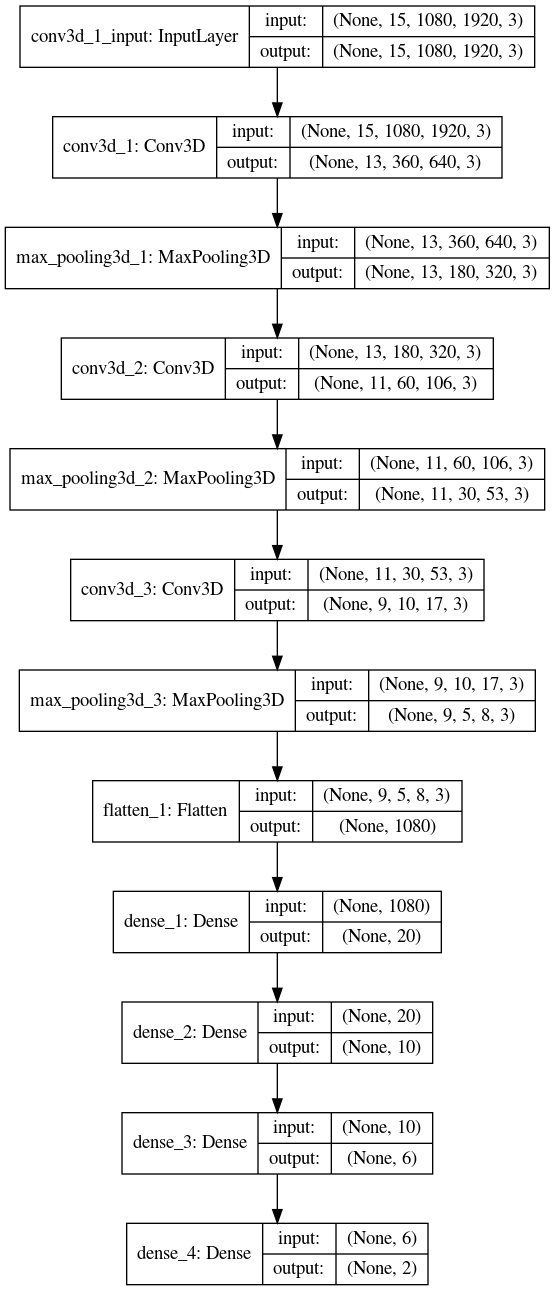
\includegraphics[width=0.5\textwidth]{first_model.png}
%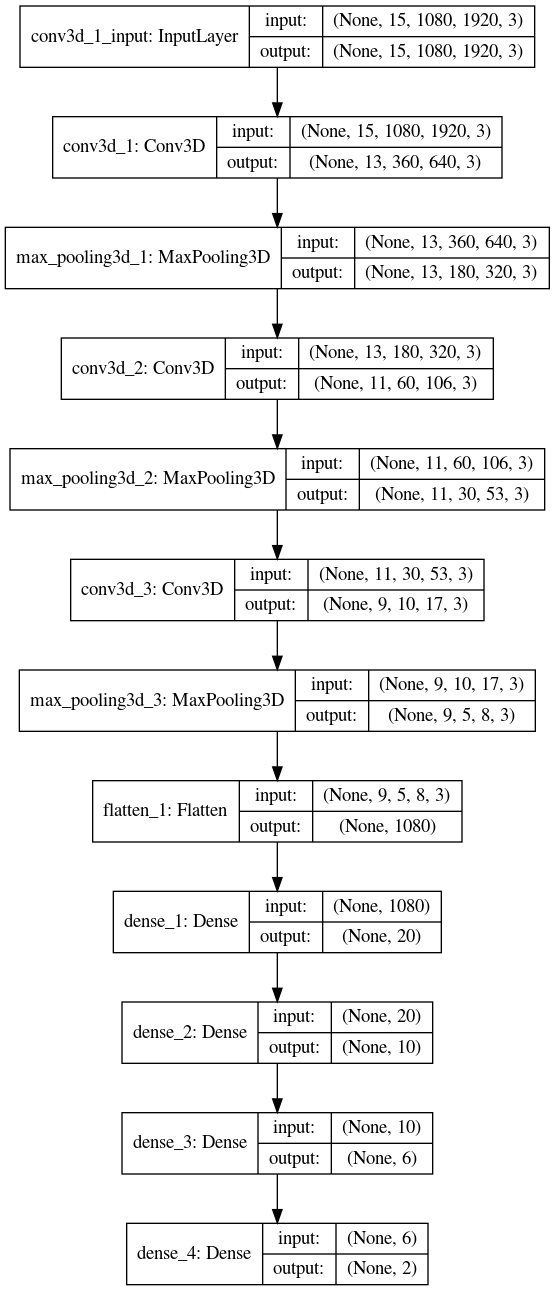
\includegraphics{first_model.png}
\end{figure}

The convolutional layers have been set with ELU activation functions.
The reason for this is to avoid dead units that emerge with ReLU activation functions
caused by 0 gradients.
For the dense layers the sigmoid activation function has been chosen.
Different activation functions could be also be investigated in the future,
such as ReLU and tanh, respectively for the convolutional and dense layers.
Also, not much tought has been given to regularization. But, since the network
seem to not fit on the training set, that's a problem for later.

\subsection{Considerations on using kernels that operate trough time}

What I noticed by watching the deepfake videos from the dataset is that some
of the videos were showing very scattered application of the face alteration.
Such abrupt changes are one of the first applications of convolutions for
image processing, such as edge detectors. Such characteristic would be 
detected here w.r.t. time.

For future reference, exclusively time-based convolution layers might be used
in a model - i.e. convolutional layers with kernel sizes that are 1 in both spatial
axes but arbitrary in the time dimension.

\subsection{Training}

Since training takes a considerable amount of time (about one hour for a training set
sweep), the number of training epochs is chosen to be as small as 100.
SGD has been chosen as optimization method. Adam/Nadam/Amsgrad/ND-Adam might be considered
as future improvement.

\subsection{Performances}
The first model is not performing well. The output category is always the most frequent 
one, which is the deepfake videos, amounting to 323, while the real videos are only 77.
This class unbalance problem could be tackled by submitting more frequently
the real videos to the training. The ratio of fake/real is 4.2, hence one possible
future improvement could be to submit about 4 different slices of the real video to 
learning for every slice of fake videos.

\end{document}
